\section{Governing equations {\&} problem setup}
\label{section:governing_equations_and_setup}
We want to ascertain the effect shape, spin, and stratification have on flow. We start by discussing how we account for stratification. We use the setup in the Nek5000 user guide\cite{fischer_nek5000_nodate}. We relate the density $\rho$ at a given position vector $\mathbf{x}$ to the constant background density $\rho_0$, $\rho = \rho_0 + \rho ' (\mathbf{x},t)$. The term $\rho'$ is the perturbation density, which we will assume to have a linear profile in the vertical direction $y$. This means the overall density distribution $\rho(\mathbf{x},t)$ has a vertical linear profile. To account for the buoyancy forces from stratification, we utilize the Boussinesq approximation. The Boussinesq approximation is where effects of density stratification are only applied to the forcing term, or terms multiplied by gravity forces in this case, in the governing equations. The Boussinesq approximation also assumes $\rho_0 \gg \rho '$.
We apply the Boussinesq approximation to the nondimensional Incompressible Navier-Stokes Equations (INSE) shown in Eqn. \ref{eq:INSE} and \ref{eq:cont}:

\begin{equation}
    \label{eq:INSE}
    \frac{\partial\mathbf{u}}{\partial t}+\mathbf{u}\cdot\nabla\mathbf{u}=-\nabla p+\frac{1}{\Rey}\nabla^2\mathbf{u}-\frac{1}{{Fr}^2} (\rho^\prime\ -\ y )\hat{y}
\end{equation}

\begin{equation}
    \label{eq:cont}
    \nabla \cdot \textbf{u} = 0
\end{equation}
We also solve the transport equation in Eqn. \ref{eq:density transport}, which is the material derivative of the perturbation density set equal to a diffusion operator.  
\begin{equation}
    \label{eq:density transport}
    \frac{\partial\rho '}{\partial t}+\mathbf{u}\cdot\nabla\rho'=\frac{1}{\Pran \Rey}\nabla^2\rho '
\end{equation}
The three nondimensional numbers that appear in the equations above are defined as such:
\[
    \Rey = \rho_0 \frac{U D}{\mu}, \Pran = \rho_0 \frac{\kappa}{\mu}, Fr^{-2}=\frac{gD^2}{\rho_0 U^2}|\rho^{\prime}_{y,0}|
\]
where $\rho^{\prime}_{y,0}$ is the density gradient, which in this case is constant. The term $U$ is the velocity scale, which is the initial flow and inflow velocity, and $D$ is the length scale, which will be discussed later. Dynamic viscosity, also known as momentum diffusivity, is represented by $\mu$, and $\kappa$ is the diffusivity of the property that is causing the stratification, which in this case is thermal diffusivity. Because the densimetric Froude term $Fr^{-2}$ is slightly clunky, often it is substituted with the Richardson number $Ri \coloneqq Fr^{-2}$. We are able to extract the physical quantity called the Brunt–Väisälä frequency defined as
\begin{equation}
    \label{eq:NBV}
    N_{BV} \coloneqq \bigg( \frac{g}{\rho_0} \rho^{\prime}_{y,0} \bigg)^{1/2}    
\end{equation}
With nondimensionality and setting $U = 1$ and $D = 1$, the Brunt–Väisälä frequency can be redefined in terms of nondimensional parameters to yield the relationship Eqn. \ref{eq:nondim NBV}:
\begin{equation}
    \label{eq:nondim NBV}
    N_{BV} = Ri^{1/2} = Fr^{-1}
\end{equation}
We observe that with higher stratification, we get higher frequencies of oscillation.
 
To understand the effect of shape, we look at three different aspect ratios ($AR$). A circle is included to allow for benchmarking purposes with literature since a sufficient number of studies have looked at spinning circles. It is shown that the horizontal dimension, $a_x$, of the body is held constant, and this dimension is what is used for the length scale in the Reynolds number $\Rey = \rho_0 \frac{U D}{\mu}$ , where $D = 2a_x$. The other dimension $a_y$ is varied to achieve the different aspect ratios. The aspect ratio is defined as $AR = a_y/a_x$. Figure \ref{fig:flow setup} shows the aspect ratios of interest for this study. 
Now we introduce spin into our setup. We follow the conventions of Mittal et al. in their 2020 \textit{Computers and Fluids} paper \cite{mittal_direct_2020} and define our nondimensional rotational velocity, also known as velocity ratio, as $\Omega^{\ast} = \tilde{\Omega}D/2 U_{\infty}$, where $\tilde{\Omega}$ is the rotational velocity in radians per unit time, and the derivative of angular displacement $\theta$. Figure \ref{fig:flow setup} shows how the ambient flow, rotation, and axes are related. The axis of rotation, which in this case is along the out-of-plane z-axis, is normal to the flow. The flow occurs along the x-direction. 
\begin{figure}
    \centerline{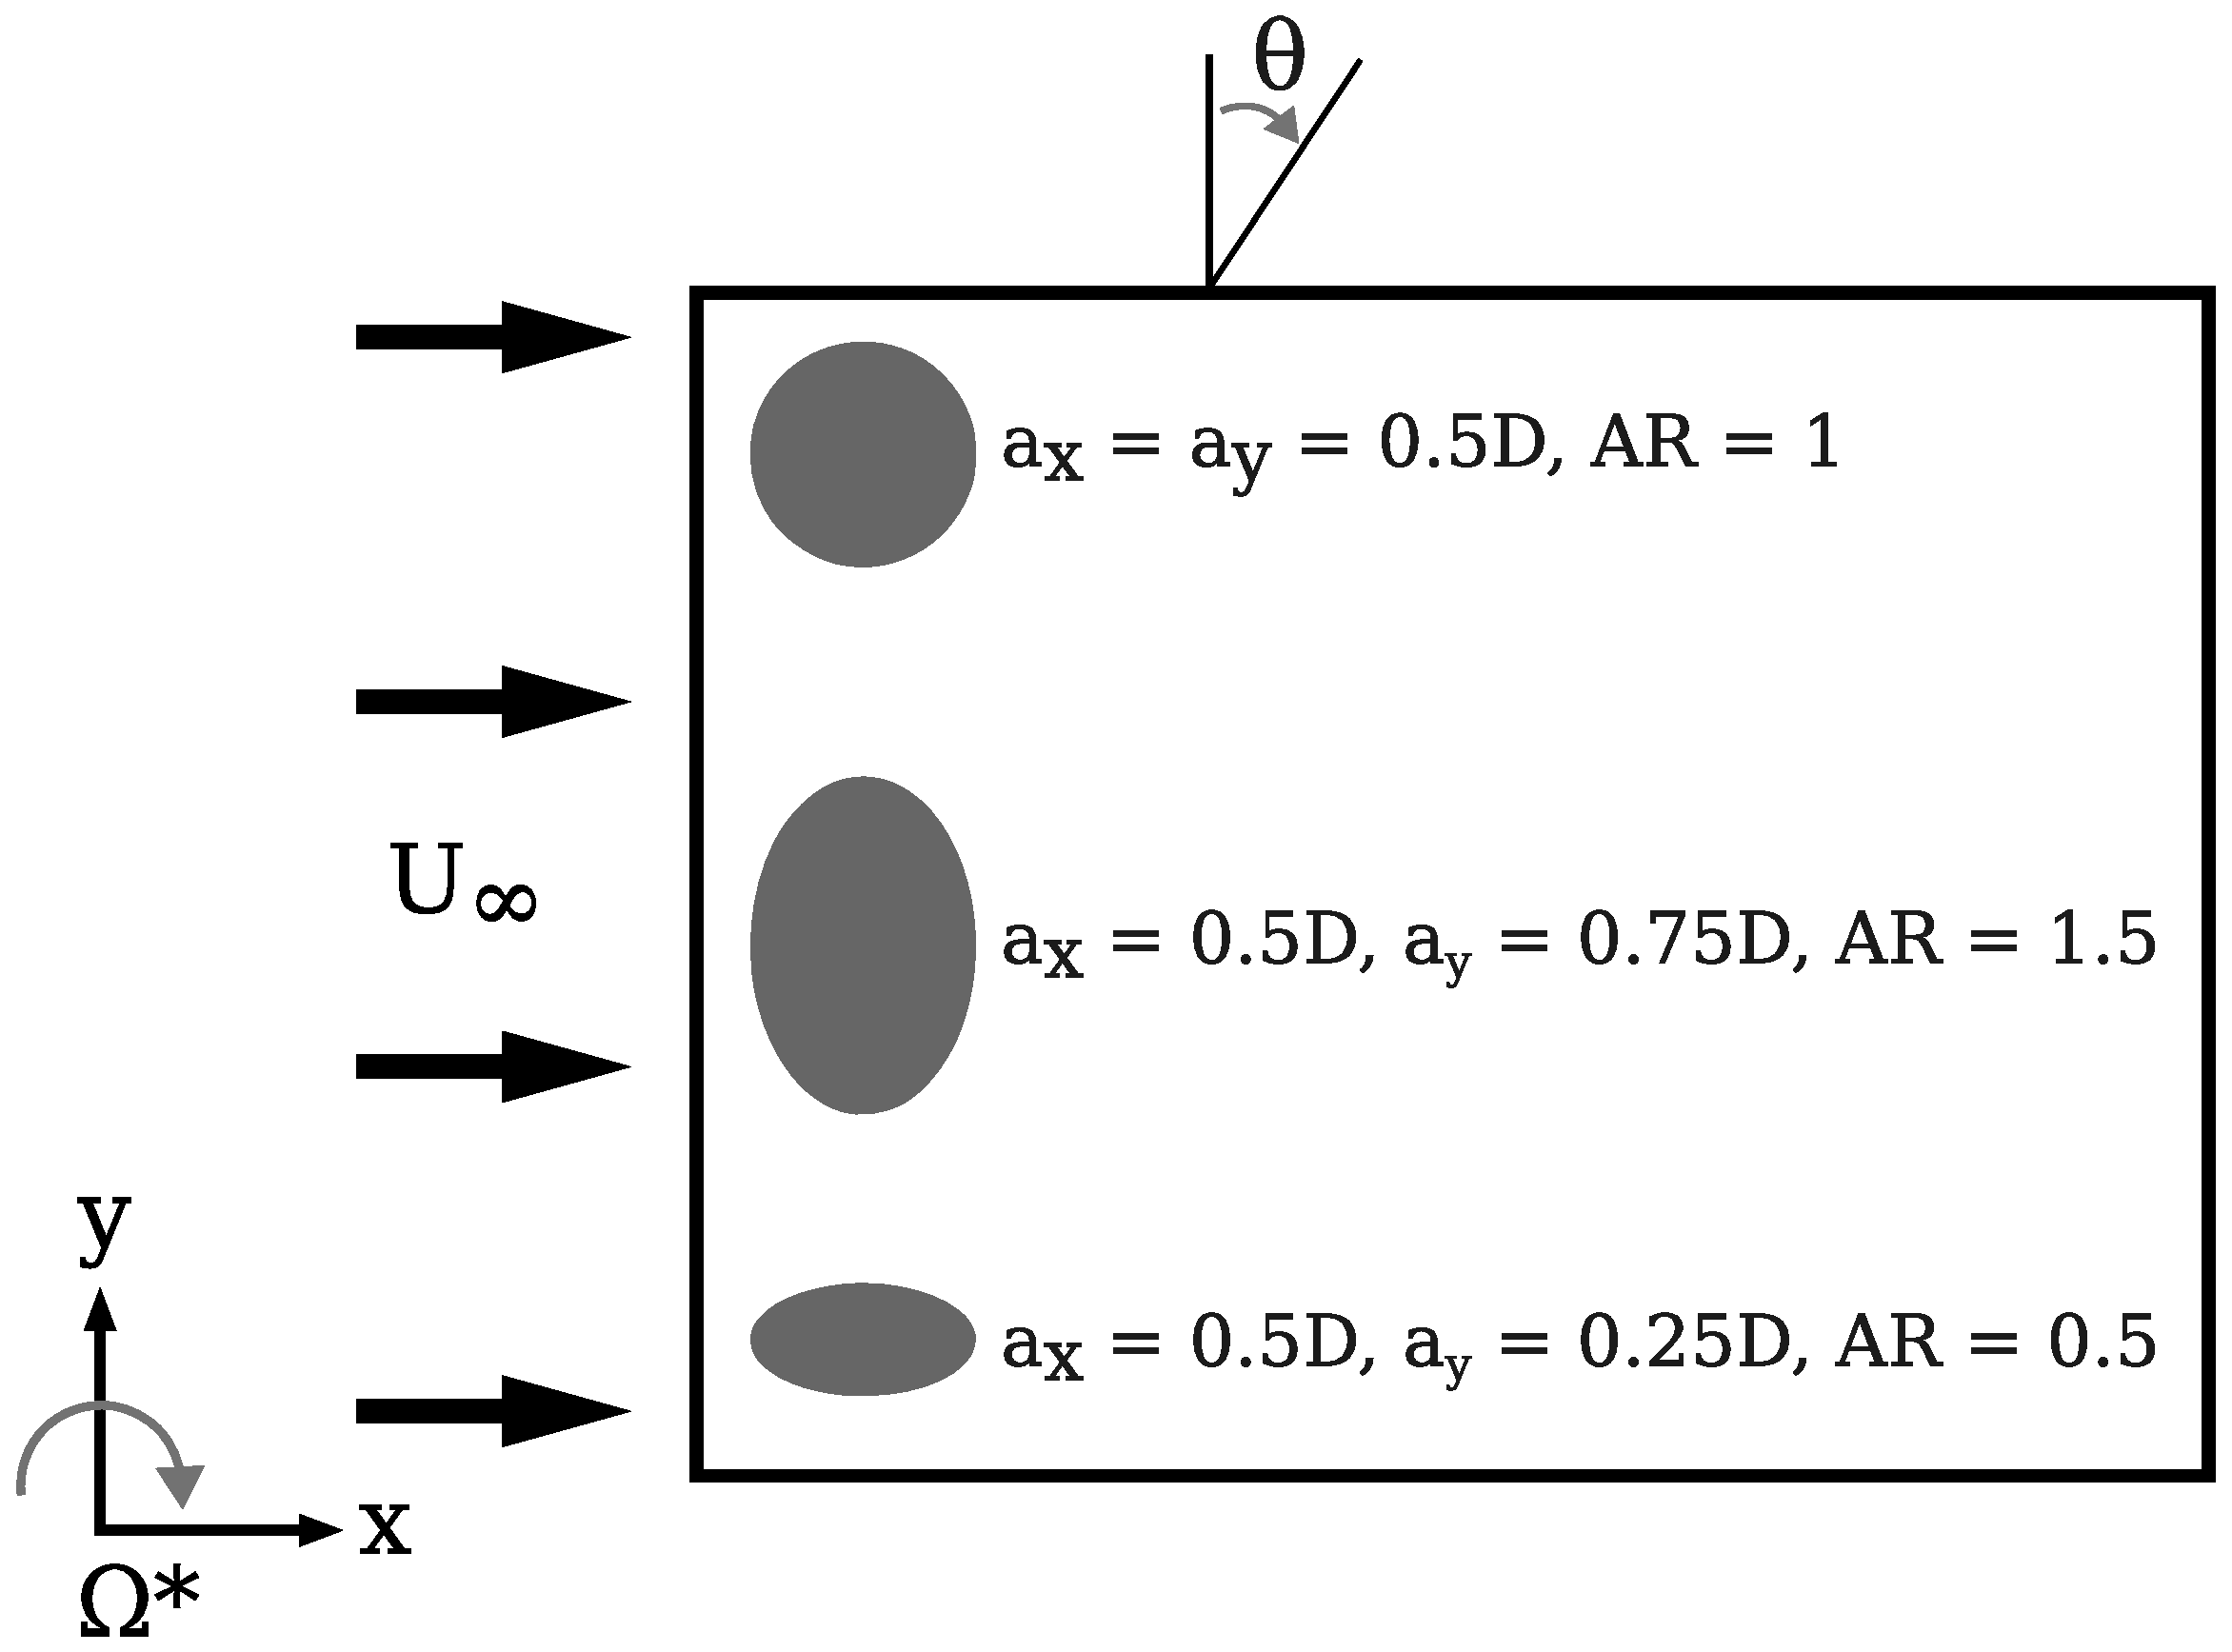
\includegraphics[width=.6\textwidth]{flow_setup.eps}}
    \caption{Schematic showing aspect ratios of interest}
    \label{fig:flow setup}
\end{figure}

This study utilizes spectral element methods (SEM) to perform direct numerical simulations (DNS). These methods allow for higher-order accuracy than methods used in past studies. Lagrange interpolants with Gauss-Lobatto-Legendre (GLL) quadrature are utilized. 
We consider cases at $\Rey = 120$. We do not go much higher than $\Rey = 120$ because at $\Rey >190$ flow regimes, 2D simulations do not sufficiently capture the flow features observed in 3D simulations \cite{deng_drag_2022}. We do not go to smaller $\Rey$ because the flows of interest occur at $\Rey > 100$. We run simulations where the stratification is a result of a linear temperature distribution, and we run simulations at a constant $\Pran = 1$. The rates of rotation of interest we will consider are $\Omega^{\ast} = 0, 1$. We compare cases with spin and no spin to observe what effect spin has on the flow. Table \ref{table:parameter_space} gives the values of our parameter sweep. A few simulations will be run with intermediate parameters not included in the aforementioned parameter values to explore transitional flow regimes. 
\begin{table}
  \centering
  \begin{tabular}{cc}
    Parameters      & Values   \\ \hline
    $AR$   & $0.5, 1.0, 1.5$ \\
    $Fr^2$ & $0.01, 0.1, 1.0, 10.0, 100.0, \infty$     \\
    $\Rey$ & $120$  \\
    $\Omega^{\ast}$ & $0.0$ (AR = 1 \text{only}), $1.0$  \\
  \end{tabular}
  \caption{The values of interest for our parameter sweep}
  \label{table:parameter_space}
\end{table}

